\documentclass[11pt,a4paper]{article}

%=============================================================================
% ENCODING AND FONTS
%=============================================================================
\usepackage[utf8]{inputenc}
\usepackage[T1]{fontenc}

%=============================================================================
% PAGE LAYOUT AND TYPOGRAPHY
%=============================================================================
\usepackage[a4paper, margin=1in]{geometry}

%=============================================================================
% HEADER AND FOOTER
%=============================================================================
\usepackage{fancyhdr}
\pagestyle{fancy}
\lhead{\experimenttitle}
\rhead{}
\cfoot{\thepage}
\renewcommand{\headrulewidth}{0.4pt}

%=============================================================================
% MATH
%=============================================================================
\usepackage{amsmath}
\usepackage{amssymb}

%=============================================================================
% GRAPHICS AND FIGURES
%=============================================================================
\usepackage{graphicx}
\usepackage{float}
\usepackage[font=small,labelfont=bf]{caption}

%=============================================================================
% TABLES
%=============================================================================
\usepackage{booktabs}
\usepackage{array}
\usepackage{multirow}
\usepackage{tabularx}

%=============================================================================
% LISTS
%=============================================================================
\usepackage{enumitem}

%=============================================================================
% COLORS
%=============================================================================
\usepackage{xcolor}
\definecolor{linkblue}{RGB}{0,51,153}

%=============================================================================
% PLOTTING
%=============================================================================
\usepackage{pgfplots}
\pgfplotsset{compat=1.18}
\usepackage{tikz}
\usetikzlibrary{shapes.geometric, arrows.meta, positioning, shadows}

%=============================================================================
% CODE LISTINGS
%=============================================================================
\usepackage{listings}
\lstset{
    basicstyle=\ttfamily\small,
    breaklines=true,
    frame=single,
    backgroundcolor=\color{gray!10},
    columns=fullflexible,
    keepspaces=true
}

%=============================================================================
% HYPERLINKS (load near end)
%=============================================================================
\usepackage{hyperref}
\hypersetup{
    colorlinks=true,
    linkcolor=linkblue,
    citecolor=linkblue,
    urlcolor=linkblue,
    pdftitle={Hand Gesture Recognition Lab Report},
    pdfauthor={Dinh Thanh Hieu, Nguyen Thai Nhat Anh, Le Quoc Anh},
    bookmarks=true
}

%=============================================================================
% DOCUMENT METADATA
%=============================================================================
\newcommand{\experimenttitle}{Hand Gesture Recognition for Puzzle Game Control}
\newcommand{\coursename}{Computer Vision}
\newcommand{\studentname}{
    \begin{tabular}{ll}
        \textbf{Dinh Thanh Hieu} & \textbf{22BA13132} \\
        \textbf{Nguyen Thai Nhat Anh} & \textbf{23BI14024} \\
        \textbf{Le Quoc Anh} & \textbf{23BI14025}
    \end{tabular}
}
\newcommand{\studentid}{}
\newcommand{\instructor}{
    \textbf{Instructor:} Prof. Nguyen Duc Dung \\
    Vietnam Academy of Science and Technology \\
    University of Science and Technology of Hanoi
}
\newcommand{\dateperformed}{Date Performed: February 2026}
\newcommand{\datesubmitted}{Date Submitted: February 2026}

%=============================================================================
% DOCUMENT
%=============================================================================
\begin{document}

% --- TITLE PAGE ---
\begin{titlepage}
    \centering
    
\includegraphics[width=0.4\textwidth]{usth_logo.png}\par
    \vspace{1.5cm}

    {\LARGE\bfseries \experimenttitle\par}
    \vspace{0.8cm}
    {\large A Comparative Study of Heuristic, Classical ML,\\and Deep Learning Approaches\par}
    \vspace{1.5cm}

    {\Large \coursename\par}
    \vspace{1.5cm}

    {\large
    \studentname\\
    \vspace{1.5cm}
    \instructor\\
    \vspace{1.5cm}
    \dateperformed\\
    \datesubmitted\\
    }

    \vfill
\end{titlepage}

% --- ABSTRACT ---
\begin{abstract}
\noindent
This project implements a real-time hand gesture recognition system for controlling a browser-based jigsaw puzzle game via webcam. Using Google MediaPipe HandLandmarker to extract 21 hand landmarks per frame, we classify gestures into five categories (open hand, fist, pinch, frame, none) using three methods: a rule-based heuristic, a Random Forest classifier, and an MLP neural network. While MediaPipe natively produces 3D coordinates $(x, y, z)$, our training benchmark uses the HaGRID v2 dataset which provides only 2D annotations ($z = 0$); the z-coordinates are retained as zero-padded dimensions for pipeline compatibility with live webcam inference. Evaluation on HaGRID v2 (9,231 samples, 3,607 unique subjects) with Group 5-Fold Cross-Validation shows that the MLP achieves 98.41\% accuracy ($\pm$0.26\%), the Random Forest achieves 94.13\% ($\pm$1.25\%), while the heuristic classifier achieves only 0.99\% due to calibration mismatch with the 2D data source. The MLP achieves the highest classification accuracy, while the Random Forest offers the best accuracy--latency tradeoff within the 60 FPS real-time budget.

\vspace{0.5cm}
\noindent
\textbf{Source Code:} \href{https://github.com/dige04/CVsubject-USTH}{https://github.com/dige04/CVsubject-USTH}
\end{abstract}

\newpage
\tableofcontents
\newpage

%=============================================================================
% INTRODUCTION
%=============================================================================
\section{Introduction}
\label{sec:intro}

Hand gesture recognition is a key research area in computer vision and human--computer interaction. This project investigates three classification approaches for recognizing hand gestures from webcam video to control a browser-based jigsaw puzzle game.

\subsection{Background and Motivation}

Human-computer interaction has traditionally relied on physical peripherals (keyboards, mice, controllers) that intermediate the user's intent. While precise, these input mechanisms tether users to workstations and are poorly suited for immersive environments. Hand gesture recognition provides a biological, touchless alternative that leverages the natural spatial dexterity of human hands.

The core motivation for this project lies in moving beyond synthetic "laboratory" constraints to real-world generalization. The physical appearance of a gesture varies dramatically across subjects depending on hand morphology (finger length, joint flexibility), skin tone, and environmental conditions (lighting, background clutter, camera angle). A robust system cannot simply memorize the geometry of a single user's hand; it must extract structural invariances. This report details the engineering of such a system, targeting real-time performance (60 FPS rendering budget) by bridging MediaPipe landmark extraction with optimal downstream classifiers.

\subsection{Objectives}

The objectives of this project are:
\begin{enumerate}
    \item Implement and compare three gesture classification methods of increasing complexity: rule-based heuristic, classical machine learning (Random Forest), and deep learning (MLP neural network).
    \item Evaluate all methods using person-aware cross-validation on a large-scale public dataset.
    \item Deploy the best-performing model in a real-time browser-based game application.
\end{enumerate}

\subsection{Gesture Classes}

Five gesture classes are defined for game control:

\begin{table}[H]
\centering
\caption{Gesture classes and their game actions.}
\label{tab:gestures}
\begin{tabular}{@{}llll@{}}
\toprule
\textbf{Gesture} & \textbf{Description} & \textbf{Game Action} \\
\midrule
Open Hand & Spread fingers, palm facing camera & Release puzzle piece \\
Fist & Closed fist & Rotate puzzle piece \\
Pinch & Thumb and index finger touching & Grab/release piece \\
Frame & Two hands forming rectangle & Take screenshot \\
None & No specific gesture & No action \\
\bottomrule
\end{tabular}
\end{table}

\subsection{Theoretical Background}

The system pipeline consists of two stages:

\begin{equation}
\label{eq:pipeline}
\text{Video Frame} \xrightarrow{\text{MediaPipe}} \mathbf{L} \in \mathbb{R}^{21 \times 3} \xrightarrow{\text{Classifier}} y \in \{1, \ldots, 5\}
\end{equation}

where $\mathbf{L}$ represents the 21 hand landmarks with $(x, y, z)$ coordinates, and $y$ is the predicted gesture class.

\subsubsection{MediaPipe Hand Landmark Detection}

MediaPipe Hands [2] is a real-time hand tracking solution developed by Google that implements a two-stage convolutional neural network (CNN) pipeline:

\begin{enumerate}
    \item \textbf{Stage 1 --- Palm Detection:} A lightweight Single Shot Detector (SSD) CNN scans the full video frame to locate the bounding box of the hand. This detector uses a modified MobileNetV2 backbone optimized for mobile inference. It runs on every frame during initial detection, and is re-triggered only when tracking confidence drops below a threshold.
    \item \textbf{Stage 2 --- Landmark Regression:} A specialized regression CNN takes the cropped hand region from Stage 1 and predicts the $(x, y, z)$ coordinates of all 21 keypoints simultaneously. This is not a classical feature detector (e.g., SIFT, ORB); instead, it is a deep regression head trained on a large-scale annotated dataset of hand poses.
    \item \textbf{Tracking Optimization:} After initial detection, MediaPipe tracks the hand across subsequent frames using the previous landmark positions as a prior, avoiding the cost of re-running the palm detector on every frame. This enables real-time performance at 30+ FPS on mobile devices.
\end{enumerate}

\subsubsection{Image Preprocessing within MediaPipe}

Before the CNN stages execute, MediaPipe applies several classical image preprocessing operations internally:

\begin{itemize}
    \item \textbf{Color Space Conversion:} The input frame is converted from the camera's native BGR format (OpenCV convention) to RGB, as the neural network was trained on RGB-ordered pixel data. This is a standard computer vision operation that ensures consistent channel ordering.
    \item \textbf{Resolution Scaling:} The palm detection model operates on a fixed $256 \times 256$ input resolution. MediaPipe downscales the full video frame using bilinear interpolation while preserving the aspect ratio via letterboxing. This reduces the computational cost of the initial detection pass.
    \item \textbf{Hand Region Cropping (ROI Extraction):} Once the palm detector localizes the bounding box, MediaPipe extracts and crops the hand Region of Interest (ROI) from the original resolution frame. This cropped region is then resized to $224 \times 224$ before being fed into the landmark regression network. By operating on a tightly cropped ROI rather than the full frame, the landmark model achieves higher spatial precision with lower computational overhead.
    \item \textbf{Pixel Normalization:} All pixel values are normalized from the integer range $[0, 255]$ to floating-point $[0.0, 1.0]$ before entering the neural network, ensuring numerical stability during inference.
\end{itemize}

This two-stage architecture represents a \textbf{transfer learning} paradigm: MediaPipe's pretrained CNNs perform the heavy computer vision task of converting raw pixel data into a structured skeletal representation, while our downstream classifiers (RF, MLP) operate on this compact 63-dimensional output.

\begin{figure}[H]
\centering
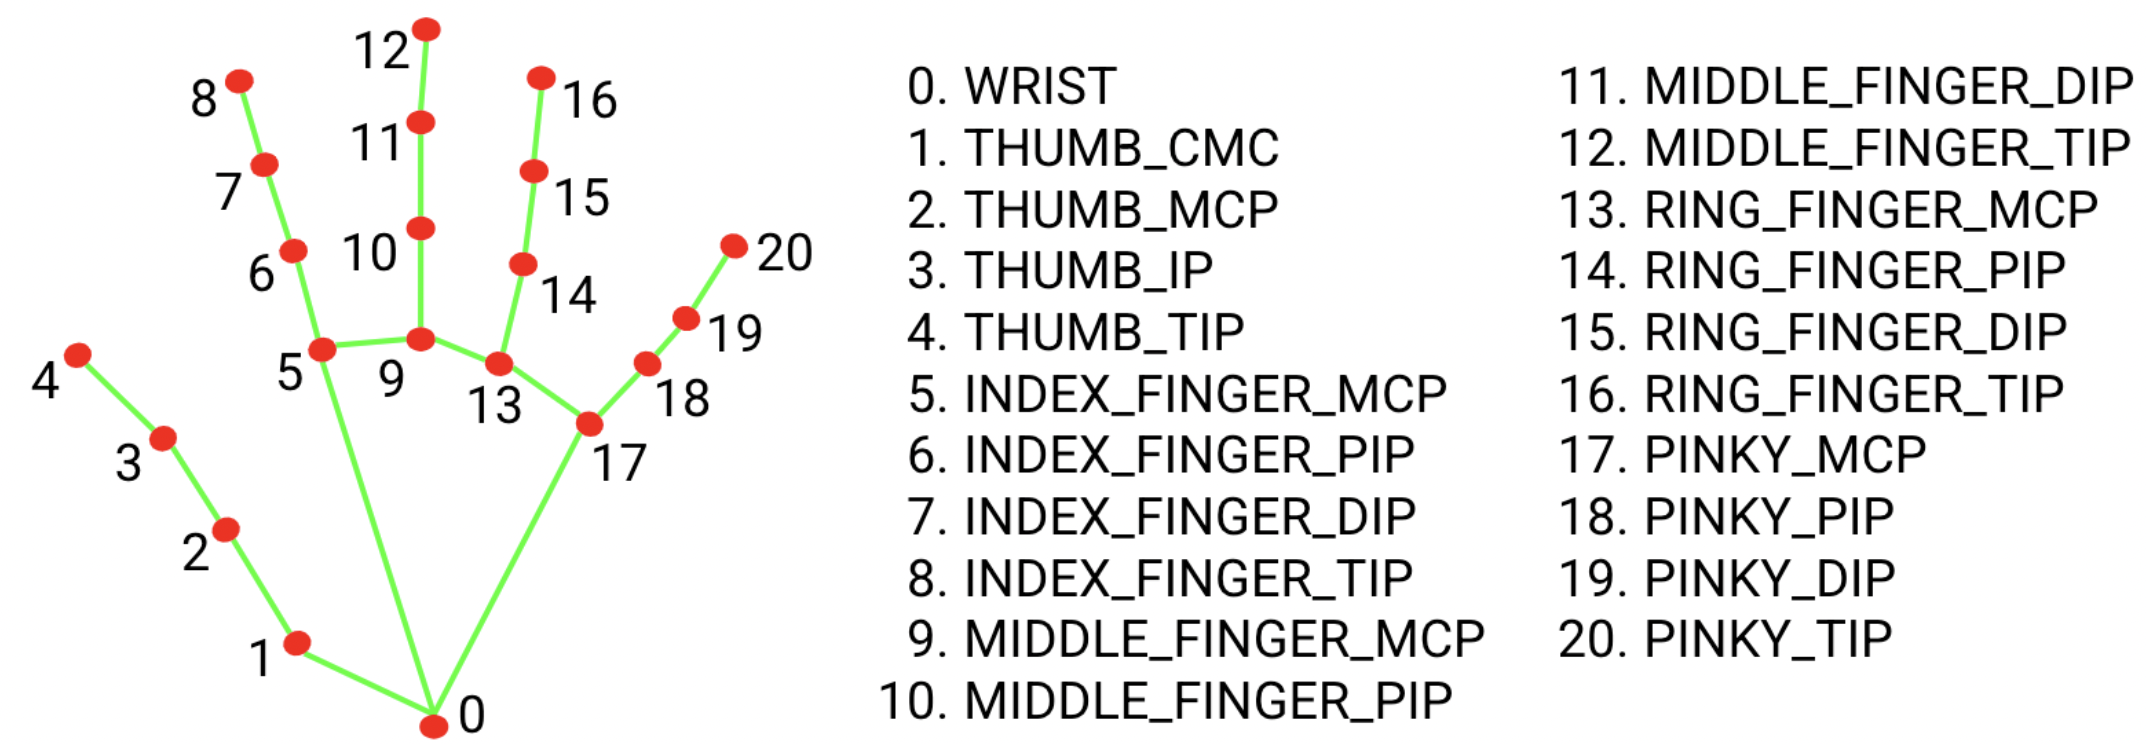
\includegraphics[width=0.6\textwidth]{mediapipe_landmarks.png}
\caption{MediaPipe hand landmark topology showing the 21 3D keypoints extracted from each hand. The wrist (joint 0) serves as the translation origin, and the middle finger MCP (joint 9) defines the scale reference distance.}
\label{fig:mediapipe-landmarks}
\end{figure}

\begin{figure}[H]
\centering
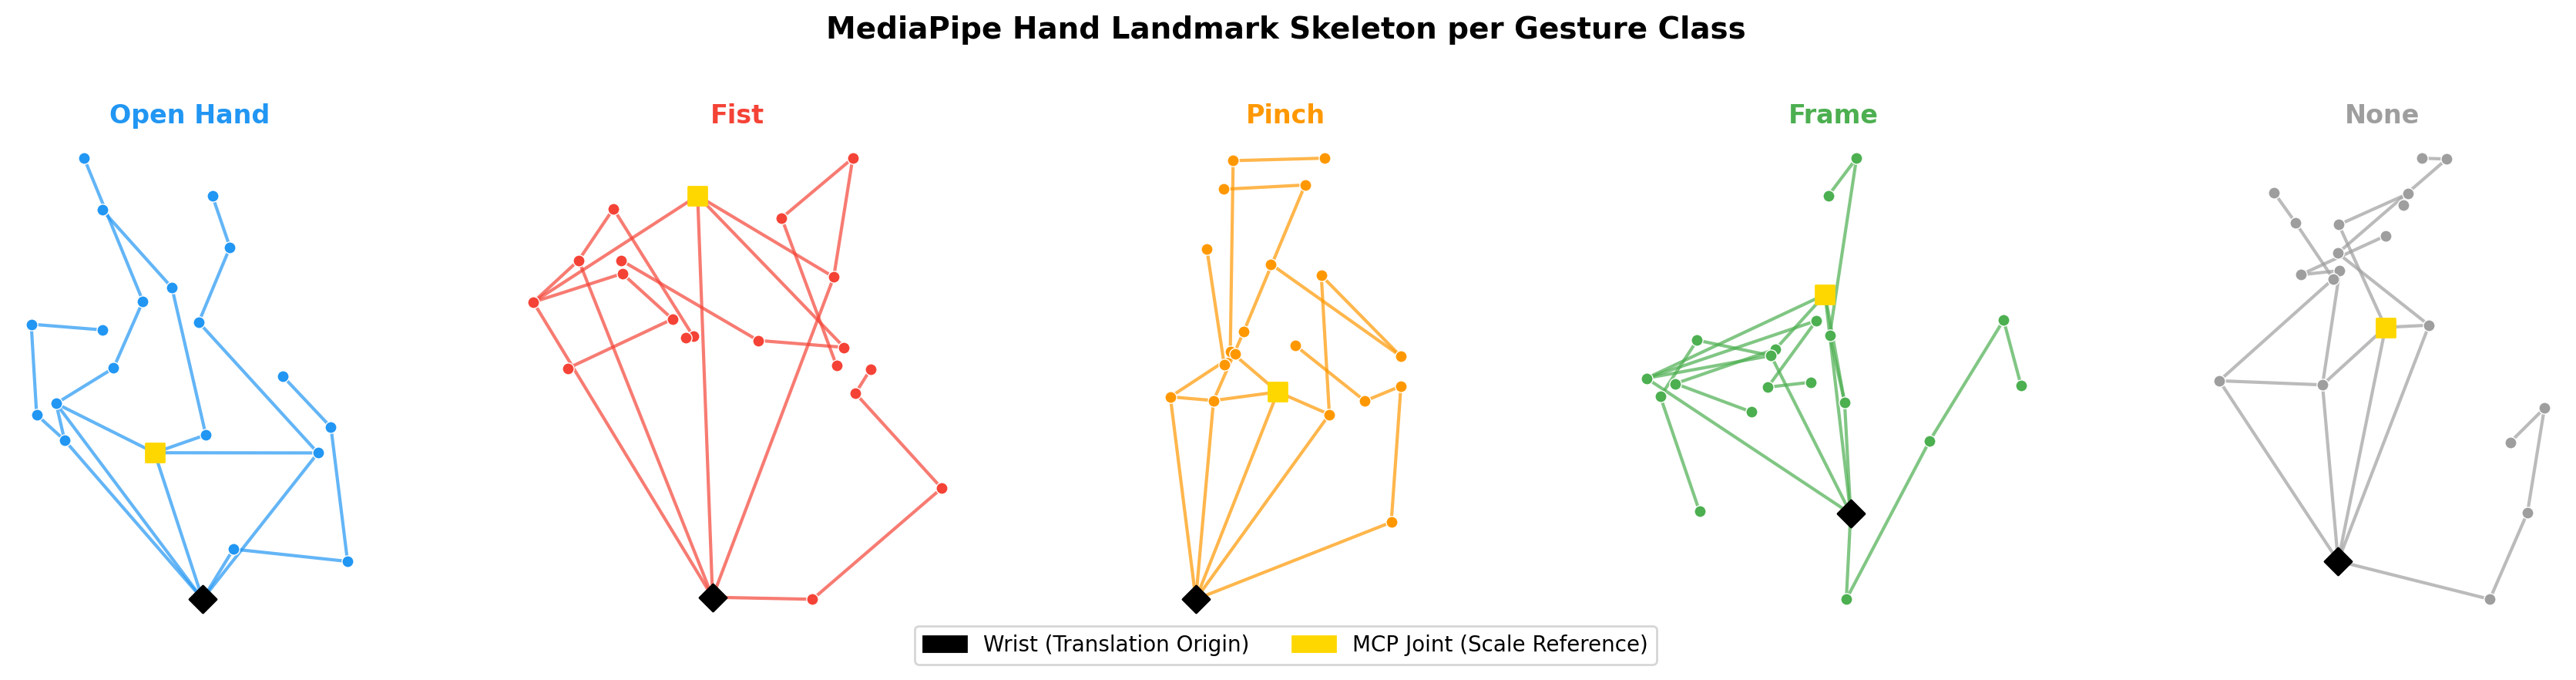
\includegraphics[width=\textwidth]{models/plots/landmark_skeleton_per_class.png}
\caption{Skeletal visualization of the 21-point hand landmark graph for each gesture class. Black diamonds mark the wrist (translation origin); gold squares mark the MCP joint (scale reference). The structural differences between gestures are clearly visible in the joint topology.}
\label{fig:landmark-skeleton}
\end{figure}

\subsection{Related Work}

Hand gesture recognition has been studied extensively using both traditional and deep learning methods.

\textbf{Landmark-based approaches.} Zhang et al.\ [3] introduced MediaPipe Hands for real-time hand tracking on mobile devices. Subsequent work has leveraged these landmarks as compact input representations, avoiding the computational cost of processing raw images. Our project follows this paradigm, using pre-extracted landmarks rather than pixel-level features.

\textbf{Classical ML on hand landmarks.} Several studies have applied Random Forest and SVM classifiers to hand landmark coordinates or derived geometric features. Pairwise distance features between landmarks have proven effective for static gesture classification, as they encode the hand's spatial configuration while being invariant to global position and orientation. Our Random Forest method (Method 2) builds on this approach with 24 selected pairwise distances.

\textbf{Neural networks for gesture recognition.} Lightweight MLPs on landmark vectors have been shown to achieve competitive accuracy with CNNs on raw images for static gesture classification, at a fraction of the computational cost. Our MLP (Method 3) uses this strategy, demonstrating that a shallow network (two hidden layers, 14,789 parameters) suffices for 5-class gesture discrimination.

\textbf{Hybrid detection approaches.} Andriyanov and Mikhailova [6] recently proposed combining MediaPipe with YOLO-Pose and XGBoost on the HaGRID dataset, using spatio-temporal features (joint angles, triangle area ratios, velocity statistics) to achieve mAP $= 0.86$ at 20 FPS. Their work demonstrates that ensembling a lightweight keypoint extractor with a full-frame object detector can improve robustness to viewing angle and gesture speed. Our approach differs by focusing on a purely landmark-based pipeline without a secondary detector, trading multi-modal detection for lower computational overhead and fully client-side browser deployment.

\textbf{The HaGRID dataset.} Kapitanov et al.\ [1] introduced HaGRID as a large-scale benchmark with 33 gesture classes from 37,583 subjects. Its scale and subject diversity make it suitable for evaluating generalization via person-aware cross-validation, which we adopt as our primary evaluation protocol.

%=============================================================================
% DATA PREPARATION
%=============================================================================
\section{Data Preparation}
\label{sec:data}

\subsection{Dataset: HaGRID v2}

We use the HaGRID v2 (Hand Gesture Recognition Image Dataset) [1], a large-scale dataset containing over 1 million FullHD RGB images across 33 gesture classes with auto-annotated MediaPipe landmarks.

Key properties:
\begin{itemize}
    \item 1,086,158 images from 37,583 unique subjects, ensuring morphological diversity.
    \item JSON annotation files provide pre-computed MediaPipe hand landmarks $(x, y)$.
    \item \textbf{Crucial limitation:} The predefined annotations provide exclusively 2-Dimensional planar data ($z=0.0$). This effectively removes depth perception from the mathematical space, fundamentally penalizing models reliant on 3D geometric computations (such as traditional Heuristics).
    \item License: CC BY-NC-SA 4.0
\end{itemize}

\begin{figure}[H]
\centering
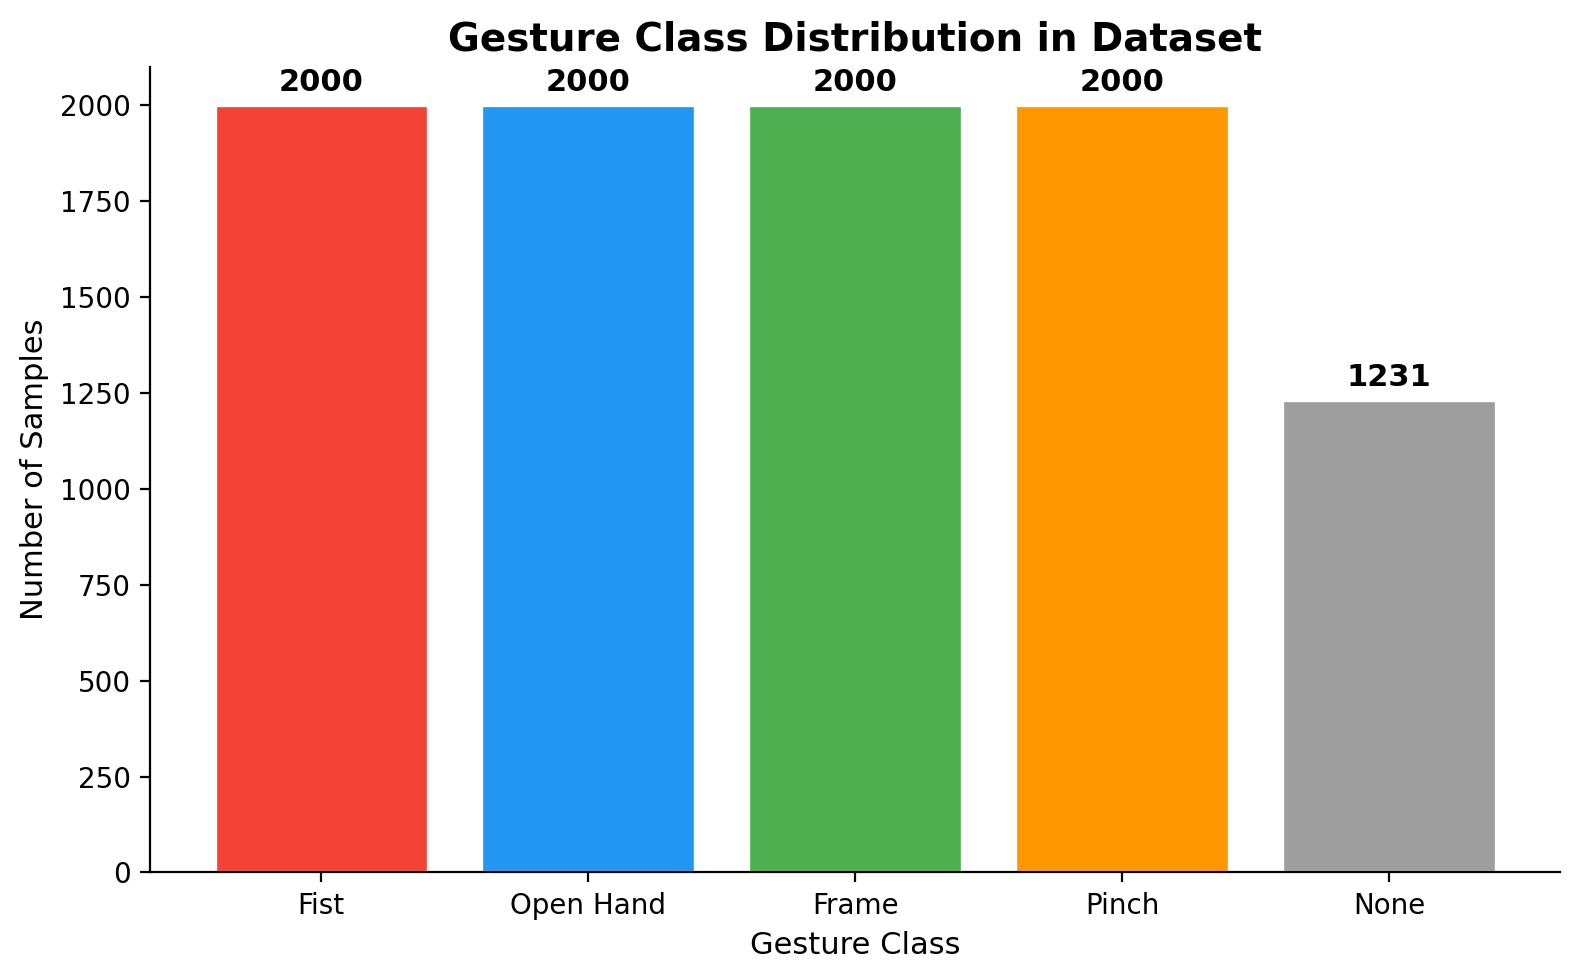
\includegraphics[width=0.7\textwidth]{models/plots/class_distribution.png}
\caption{Distribution of gesture samples across the five classes. The dataset is approximately balanced, with each class containing $\sim$2,000 samples except the ``none'' class (1,231 samples).}
\label{fig:class-distribution}
\end{figure}

\subsection{Gesture Mapping}

Five HaGRID gesture classes were mapped to our target gestures:

\begin{table}[H]
\centering
\caption{Mapping from HaGRID classes to project gesture classes.}
\label{tab:mapping}
\begin{tabular}{@{}lll@{}}
\toprule
\textbf{Our Class} & \textbf{HaGRID Class} & \textbf{Rationale} \\
\midrule
open\_hand & \texttt{stop} & Upright open hand, palm facing camera \\
fist & \texttt{fist} & Direct match \\
pinch & \texttt{thumb\_index} & Thumb and index finger touching \\
frame & \texttt{take\_picture} & Two-hand rectangular frame \\
none & \texttt{no\_gesture} & Background / no specific gesture \\
\bottomrule
\end{tabular}
\end{table}

\subsection{Data Extraction}

A conversion script (\texttt{ml/convert\_hagrid.py}) parses the HaGRID JSON annotations and extracts MediaPipe landmarks into CSV format with schema:

\begin{lstlisting}
person_id, gesture_label, timestamp, x0, y0, z0, x1, y1, z1, ..., x20, y20, z20
\end{lstlisting}

HaGRID annotations provide only $(x, y)$ coordinates. The $z$-coordinate is set to 0.0. We intentionally retain the zero-padded $z$-dimension (yielding 60D rather than 40D feature vectors) for two reasons: (a)~\textbf{pipeline consistency}---the same preprocessing code must handle both HaGRID training data and live webcam inference where MediaPipe produces real $z$-values; and (b)~\textbf{empirical validation}---the MLP learns to effectively ignore the zero $z$-channels (confirmed by near-zero weight magnitudes on $z$-input neurons), so there is no performance penalty from retaining them.

\subsection{Dataset Statistics}

\begin{table}[H]
\centering
\caption{Dataset split statistics.}
\label{tab:dataset-stats}
\begin{tabular}{@{}lrrr@{}}
\toprule
\textbf{Class} & \textbf{Train} & \textbf{Val} & \textbf{Total} \\
\midrule
open\_hand & 1,000 & 1,000 & 2,000 \\
fist & 1,000 & 1,000 & 2,000 \\
pinch & 1,000 & 1,000 & 2,000 \\
frame & 1,000 & 1,000 & 2,000 \\
none & 1,000 & 231 & 1,231 \\
\midrule
\textbf{Total} & \textbf{5,000} & \textbf{4,231} & \textbf{9,231} \\
\bottomrule
\end{tabular}
\end{table}

The dataset contains 3,607 unique subjects (from HaGRID \texttt{user\_id}). Samples were capped at 1,000 per gesture per split for computational efficiency. The mild class imbalance in the ``none'' class (1,231 vs.\ 2,000 for other classes) was intentionally left unaddressed: we did not apply oversampling (SMOTE) or class weighting because (a) the imbalance ratio (1:1.6) is within acceptable bounds for tree-based and neural network classifiers, and (b) artificially inflating the ``none'' class would risk introducing synthetic noise into an already high-variance negative class. The MLP's achieved F1 of 0.953 on ``none'' confirms that the imbalance does not materially degrade performance.

\subsection{Preprocessing Pipeline}

All methods share a common preprocessing pipeline that normalizes raw MediaPipe landmarks. Raw coordinate arrays are highly sensitive to the spatial location of the user (e.g., standing far away vs. close to the lens) and the frame region. To strip this noise and expose pure structural intent, we mandate position- and scale-invariance:

\begin{enumerate}
    \item \textbf{Wrist-relative translation (Position Invariance)}: We re-center the mathematical space so that the wrist landmark (index 0) becomes the origin coordinate $(0,0,0)$. This is achieved by subtracting the wrist vector from all 21 keypoints. This makes the models blind to \textit{where} the hand is located in the frame.
    \item \textbf{Scale normalization (Size Invariance)}: Users have substantially different hand anatomical proportions. We divide all translated coordinates by the Euclidean distance from the wrist to the middle-finger MCP joint (index 9). This standardizes the hand skeleton to a uniform unit size:
    \begin{equation}
        \hat{\mathbf{l}}_i = \frac{\mathbf{l}_i - \mathbf{l}_0}{\|\mathbf{l}_9 - \mathbf{l}_0\|_2}, \quad i = 1, \ldots, 20
    \end{equation}
    \item \textbf{Feature Array Construction}: Post-normalization, the wrist vector is effectively zeroed out and removed, yielding 20 structural landmarks $\times$ 3 coordinates. The final output passed to our algorithms is a tightly-packed \textbf{60-dimensional feature vector}.
\end{enumerate}

To validate the effectiveness of our normalization pipeline, we apply t-SNE dimensionality reduction to project the 60-dimensional feature vectors into a 2D scatter plot (Figure~\ref{fig:tsne}). The resulting clusters demonstrate that the five gesture classes are well-separated in the normalized feature space, confirming that the preprocessing successfully extracts discriminative structural information.

\begin{figure}[H]
\centering
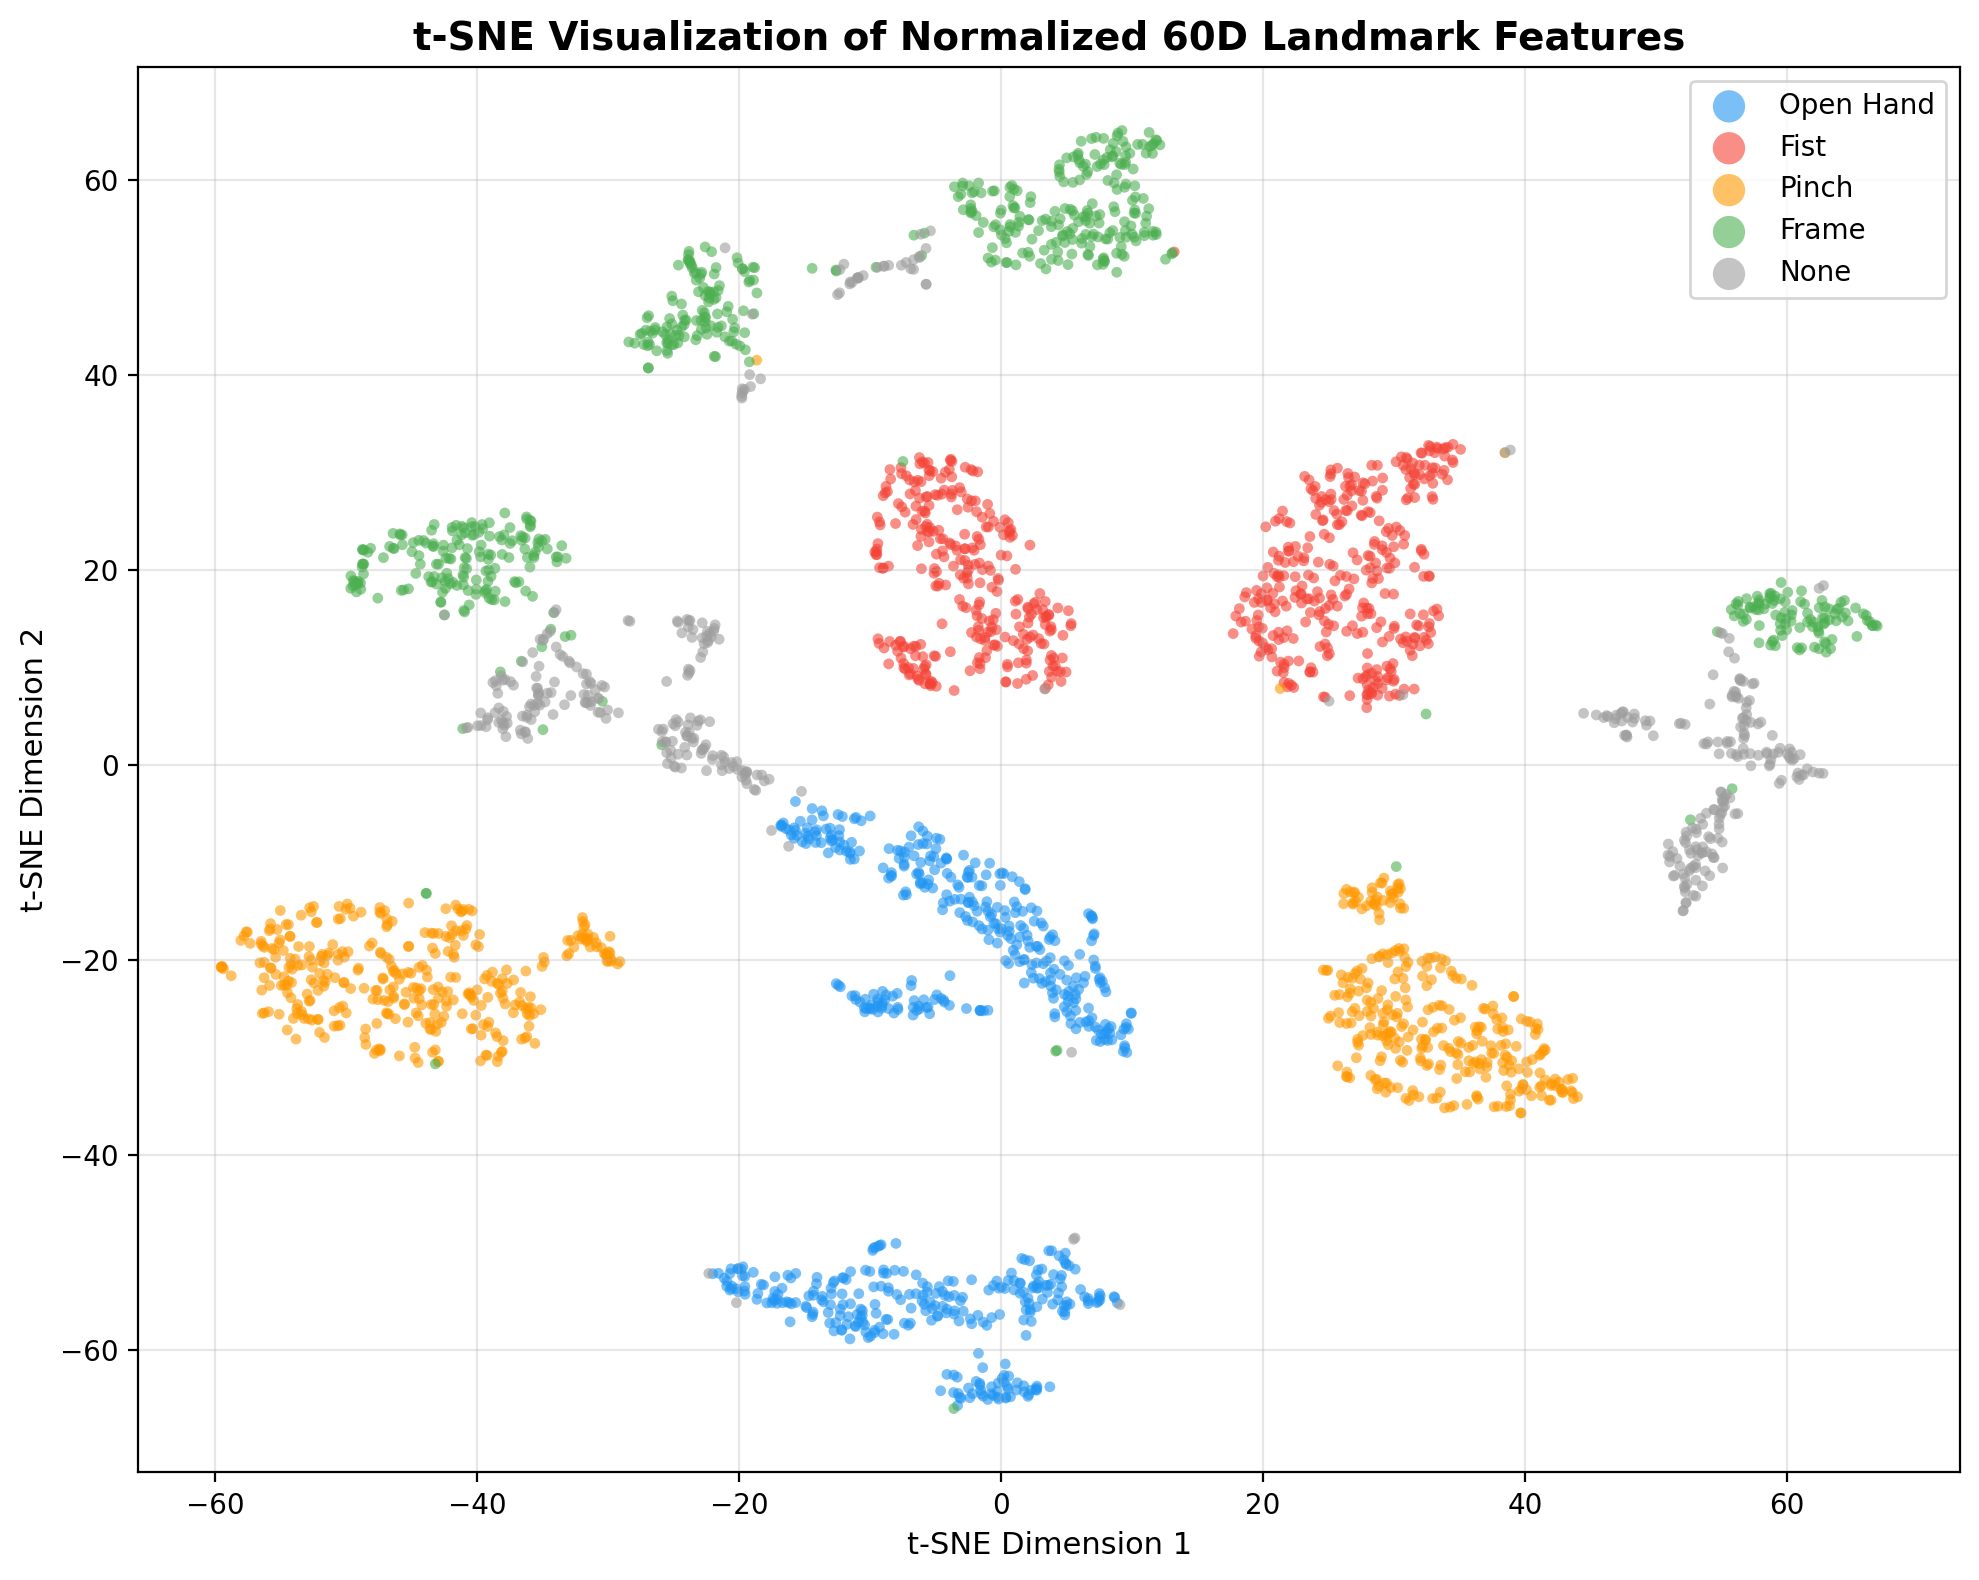
\includegraphics[width=0.75\textwidth]{models/plots/tsne_feature_space.png}
\caption{t-SNE 2D projection of the normalized 60-dimensional landmark features, colored by gesture class. Well-separated clusters validate that the normalization pipeline preserves discriminative structural information across subjects.}
\label{fig:tsne}
\end{figure}

%=============================================================================
% FEATURE EXTRACTION AND MODEL TRAINING
%=============================================================================
\section{Feature Extraction and Model Training}
\label{sec:methods}

\subsection{Method 1: Rule-Based Heuristic Classifier}

\textbf{Approach:} Hand-crafted threshold rules on geometric features computed from normalized landmarks.

\textbf{Features computed:}
\begin{itemize}
    \item \textbf{Finger curl angles}: Angle between proximal--intermediate and intermediate--distal phalange segments for each finger.
    \item \textbf{Key distances}: Fingertip-to-palm distances, inter-finger distances.
\end{itemize}

\textbf{Classification rules:}
\begin{itemize}
    \item Open Hand: All fingers extended (curl angles below threshold)
    \item Fist: All fingers curled (curl angles above threshold)
    \item Pinch: Thumb-tip to index-tip distance below proximity threshold
    \item Frame: Two hands detected with specific spatial relationship
    \item None: Default when no other rule matches
\end{itemize}

No training is required---rules are fixed a priori with approximately 20 threshold parameters.

\subsection{Method 2: Random Forest Classifier}

\textbf{Approach:} Ensemble of 100 decision trees trained on engineered pairwise distance features.

\textbf{Features (24-dimensional):} Pairwise Euclidean distances between key landmark pairs (fingertips, MCP joints, PIP joints), selected to capture discriminative geometric relationships.

\textbf{Configuration:}
\begin{itemize}
    \item \texttt{sklearn.ensemble.RandomForestClassifier}
    \item \texttt{n\_estimators=100}, \texttt{max\_depth=15}
\end{itemize}

\subsection{Method 3: MLP Neural Network}

\textbf{Approach:} Feed-forward neural network operating directly on the 60-dimensional normalized landmark vector.

\textbf{Architecture:}
\begin{equation}
\resizebox{0.9\textwidth}{!}{$\text{Input}(60) \rightarrow \text{Dense}(128, \text{ReLU}) \rightarrow \text{Drop}(0.3) \rightarrow \text{Dense}(64, \text{ReLU}) \rightarrow \text{Drop}(0.3) \rightarrow \text{Dense}(5, \text{Softmax})$}
\end{equation}

Formally, the forward pass for the hidden layers and the output layer can be expressed using matrix notation:
\begin{align}
\mathbf{h}^{(1)} &= \text{ReLU}\left(\mathbf{W}^{(1)}\mathbf{x} + \mathbf{b}^{(1)}\right) \\
\mathbf{h}^{(2)} &= \text{ReLU}\left(\mathbf{W}^{(2)}\mathbf{h}^{(1)} + \mathbf{b}^{(2)}\right) \\
\mathbf{\hat{y}} &= \text{Softmax}\left(\mathbf{W}^{(3)}\mathbf{h}^{(2)} + \mathbf{b}^{(3)}\right)
\end{align}
where $\mathbf{x} \in \mathbb{R}^{60}$ is the normalized landmark vector, $\mathbf{W}^{(1)} \in \mathbb{R}^{128 \times 60}$, $\mathbf{W}^{(2)} \in \mathbb{R}^{64 \times 128}$, and $\mathbf{W}^{(3)} \in \mathbb{R}^{5 \times 64}$ are the weight matrices, and $\mathbf{b}^{(1)}, \mathbf{b}^{(2)}, \mathbf{b}^{(3)}$ are the respective bias vectors. Dropout is applied during training after each hidden layer to prevent overfitting.

\textbf{Training configuration:}
\begin{itemize}
    \item Optimizer: Adam (learning rate $= 10^{-3}$)
    \item Loss: Sparse categorical cross-entropy
    \item Early stopping: patience = 10 epochs, monitoring validation loss
    \item Batch size: 32, maximum epochs: 50
\end{itemize}

Training converged in 17 epochs (early stopped), with train accuracy = 98.56\% and validation accuracy = 97.98\%.

\subsection{Methodology Comparison}

\begin{table}[H]
\centering
\caption{Comparison of the three classification methods.}
\label{tab:method-comparison}
\begin{tabular}{@{}llll@{}}
\toprule
\textbf{Aspect} & \textbf{Heuristic} & \textbf{Random Forest} & \textbf{MLP} \\
\midrule
Input Features & Angles + distances & 24 pairwise dist. & 60 raw coords \\
Feature Engineering & Manual & Semi-automatic & None (end-to-end) \\
Training Required & No & Yes (fast) & Yes (moderate) \\
Parameters & $\sim$20 thresholds & $\sim$100K nodes & 14,789 weights \\
Model Size & 170 B & 8.6 MB & 227 KB \\
Interpretability & High & Medium & Low \\
\bottomrule
\end{tabular}
\end{table}

%=============================================================================
% EVALUATION
%=============================================================================
\section{Evaluation}
\label{sec:evaluation}

\subsection{Experimental Setup}

All experiments were conducted on an Apple MacBook Air with an M1 chip (8-core CPU, 8-core GPU, 8\,GB unified memory) running macOS. The ML models were trained and evaluated using Python 3.11 with scikit-learn 1.5 (Random Forest), TensorFlow/Keras 2.17 (MLP), and NumPy 1.26. Inference latency was measured as the \textbf{classifier-only execution time} (excluding MediaPipe landmark extraction), averaged over 1,000 predictions on batch size~1 after a 100-iteration warm-up. This ensures a fair comparison: all three methods receive identical pre-extracted landmark vectors as input.

\subsection{Cross-Validation Strategy}

We use \textbf{Group 5-Fold Cross-Validation} (\texttt{sklearn.model\_selection.GroupKFold}) with person IDs as groups. This ensures:
\begin{itemize}
    \item No subject appears in both training and test sets within any fold
    \item The model is evaluated on truly unseen individuals
    \item Results reflect generalization to new users
\end{itemize}

We note that \texttt{GroupKFold} does not guarantee label stratification within each fold. However, our per-fold accuracy variance is low (MLP std $= 0.26\%$), indicating that class distributions remain approximately balanced across folds due to the large number of subjects (3,607). Full Leave-One-Person-Out CV was computationally impractical with 3,607 unique subjects. A stratified 80/20 split provides a secondary evaluation metric.

\subsection{Overall Results}

\begin{table}[H]
\centering
\caption{Overall classification results across all three methods.}
\label{tab:results}
\begin{tabular}{@{}lccccc@{}}
\toprule
\textbf{Method} & \textbf{CV Acc.} & \textbf{Std Dev} & \textbf{Strat. Split} & \textbf{Latency} & \textbf{95\% CI} \\
\midrule
Heuristic & 0.99\% & $\pm$0.26\% & 1.08\% & 0.1 ms & [0.78, 1.18]\% \\
Random Forest & 94.13\% & $\pm$1.25\% & 95.29\% & 13.2 ms & [93.65, 94.57]\% \\
\textbf{MLP} & \textbf{98.41\%} & $\pm$\textbf{0.26\%} & \textbf{98.75\%} & 43.7 ms & [98.16, 98.64]\% \\
\bottomrule
\end{tabular}
\end{table}

\subsection{Per-Class Results: Random Forest}

\begin{table}[H]
\centering
\caption{Per-class metrics for Random Forest (94.13\% overall).}
\label{tab:rf-perclass}
\begin{tabular}{@{}lcccc@{}}
\toprule
\textbf{Class} & \textbf{Precision} & \textbf{Recall} & \textbf{F1-Score} & \textbf{Support} \\
\midrule
open\_hand & 0.984 & 0.986 & 0.985 & 2,000 \\
fist & 0.976 & 0.990 & 0.983 & 2,000 \\
pinch & 0.935 & 0.903 & 0.919 & 2,000 \\
frame & 0.898 & 0.887 & 0.892 & 2,000 \\
none & 0.898 & 0.941 & 0.919 & 1,231 \\
\bottomrule
\end{tabular}
\end{table}

\subsection{Per-Class Results: MLP}

\begin{table}[H]
\centering
\caption{Per-class metrics for MLP (98.41\% overall).}
\label{tab:mlp-perclass}
\begin{tabular}{@{}lcccc@{}}
\toprule
\textbf{Class} & \textbf{Precision} & \textbf{Recall} & \textbf{F1-Score} & \textbf{Support} \\
\midrule
open\_hand & 0.989 & 0.999 & 0.994 & 2,000 \\
fist & 0.992 & 0.994 & 0.993 & 2,000 \\
pinch & 0.995 & 0.995 & 0.995 & 2,000 \\
frame & 0.981 & 0.966 & 0.973 & 2,000 \\
none & 0.951 & 0.956 & 0.953 & 1,231 \\
\bottomrule
\end{tabular}
\end{table}

\subsection{Cross-Validation Fold Stability}

\begin{table}[H]
\centering
\caption{Accuracy per fold for Group 5-Fold CV.}
\label{tab:cv-folds}
\begin{tabular}{@{}lccc@{}}
\toprule
\textbf{Fold} & \textbf{Heuristic} & \textbf{Random Forest} & \textbf{MLP} \\
\midrule
1 & 0.60\% & 93.45\% & 98.48\% \\
2 & 0.98\% & 94.64\% & 97.89\% \\
3 & 1.30\% & 94.75\% & 98.54\% \\
4 & 1.25\% & 92.09\% & 98.54\% \\
5 & 0.81\% & 95.72\% & 98.59\% \\
\bottomrule
\end{tabular}
\end{table}

The MLP shows stable performance across folds (std = 0.26\%), indicating strong generalization. The Random Forest shows slightly more variance (std = 1.25\%), particularly on fold 4.

\subsection{Accuracy vs.\ Latency Tradeoff}

\begin{figure}[H]
\centering
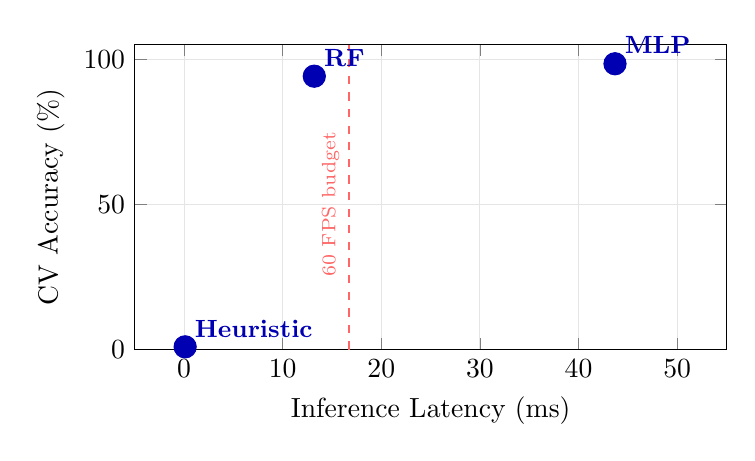
\begin{tikzpicture}
\begin{axis}[
    width=0.75\textwidth,
    height=0.45\textwidth,
    xlabel={Inference Latency (ms)},
    ylabel={CV Accuracy (\%)},
    xmin=-5, xmax=55,
    ymin=0, ymax=105,
    grid=major,
    major grid style={thin, gray!20},
    legend pos=south east,
    nodes near coords,
    nodes near coords style={font=\small\bfseries, anchor=south west},
    point meta=explicit symbolic,
]
\addplot[
    only marks,
    mark=*,
    mark size=4pt,
    color=blue!70!black,
] coordinates {
    (0.1, 0.99) [Heuristic]
    (13.2, 94.13) [RF]
    (43.7, 98.41) [MLP]
};

% 60 FPS budget line
\draw[dashed, red!60, thick] (axis cs:16.7, 0) -- (axis cs:16.7, 105);
\node[rotate=90, anchor=south, font=\scriptsize, red!60] at (axis cs:16.7, 50) {60 FPS budget};

\end{axis}
\end{tikzpicture}
\caption{Accuracy vs.\ inference latency for the three methods. The dashed line indicates the 16.7\,ms budget for 60 FPS rendering.}
\label{fig:accuracy-latency}
\end{figure}

\subsection{Confusion Matrices}

\begin{figure}[H]
\centering
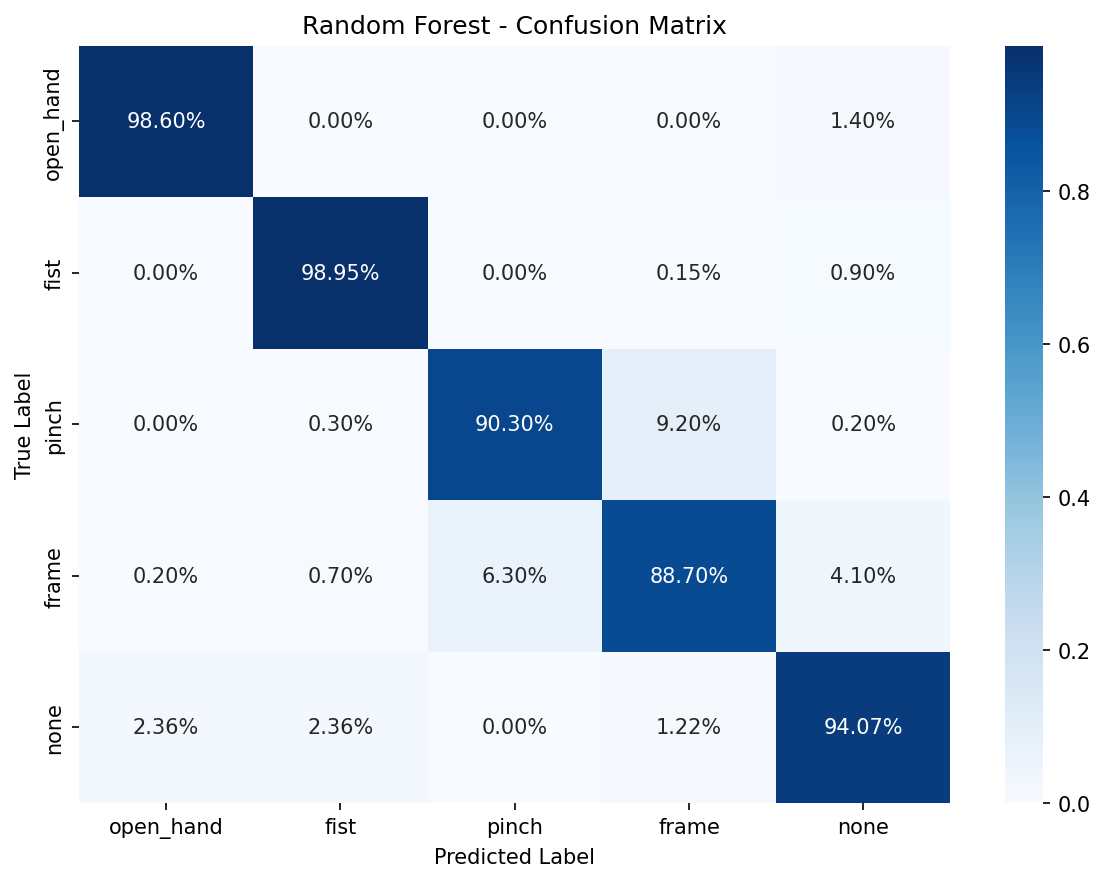
\includegraphics[width=0.75\textwidth]{models/plots/rf_confusion_matrix.png}
\caption{Confusion matrix for the Random Forest classifier. Frame and pinch gestures show the highest confusion rates.}
\label{fig:rf-cm}
\end{figure}

\begin{figure}[H]
\centering
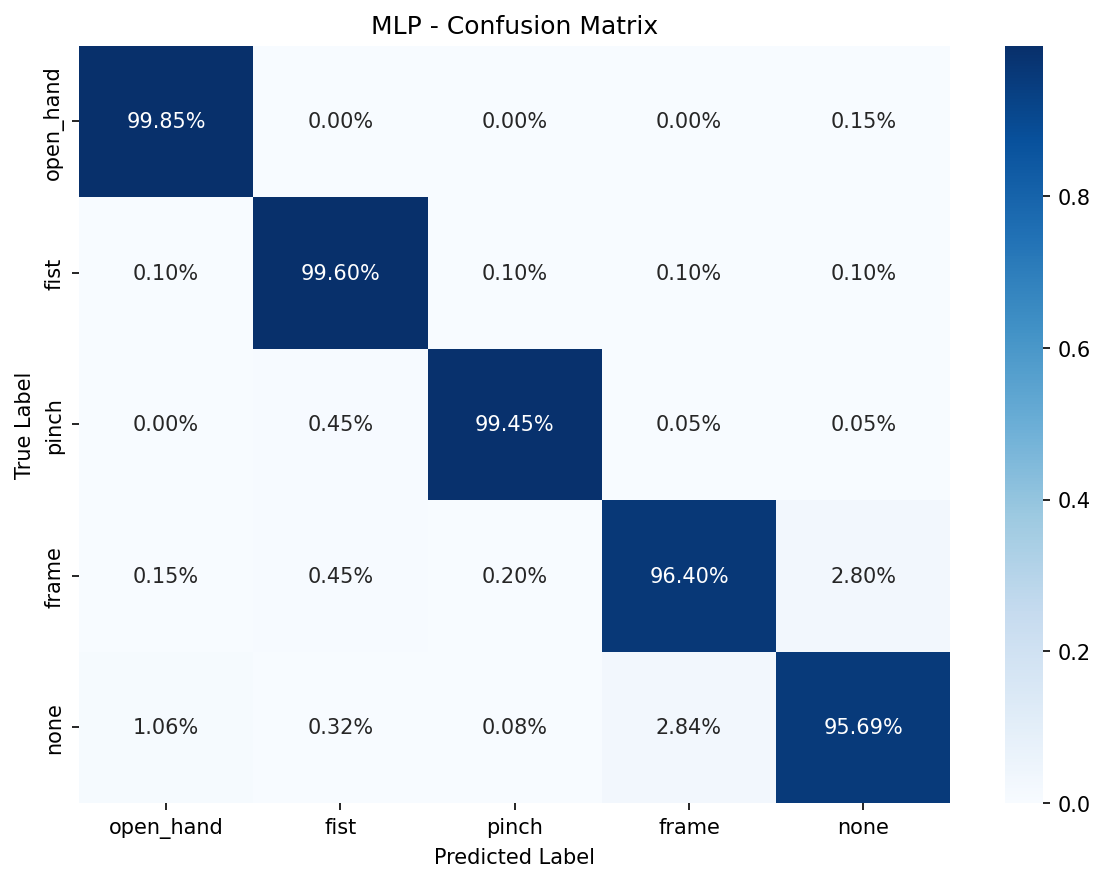
\includegraphics[width=0.75\textwidth]{models/plots/mlp_confusion_matrix.png}
\caption{Confusion matrix for the MLP classifier. All classes achieve $>$95\% recall.}
\label{fig:mlp-cm}
\end{figure}

\begin{figure}[H]
\centering
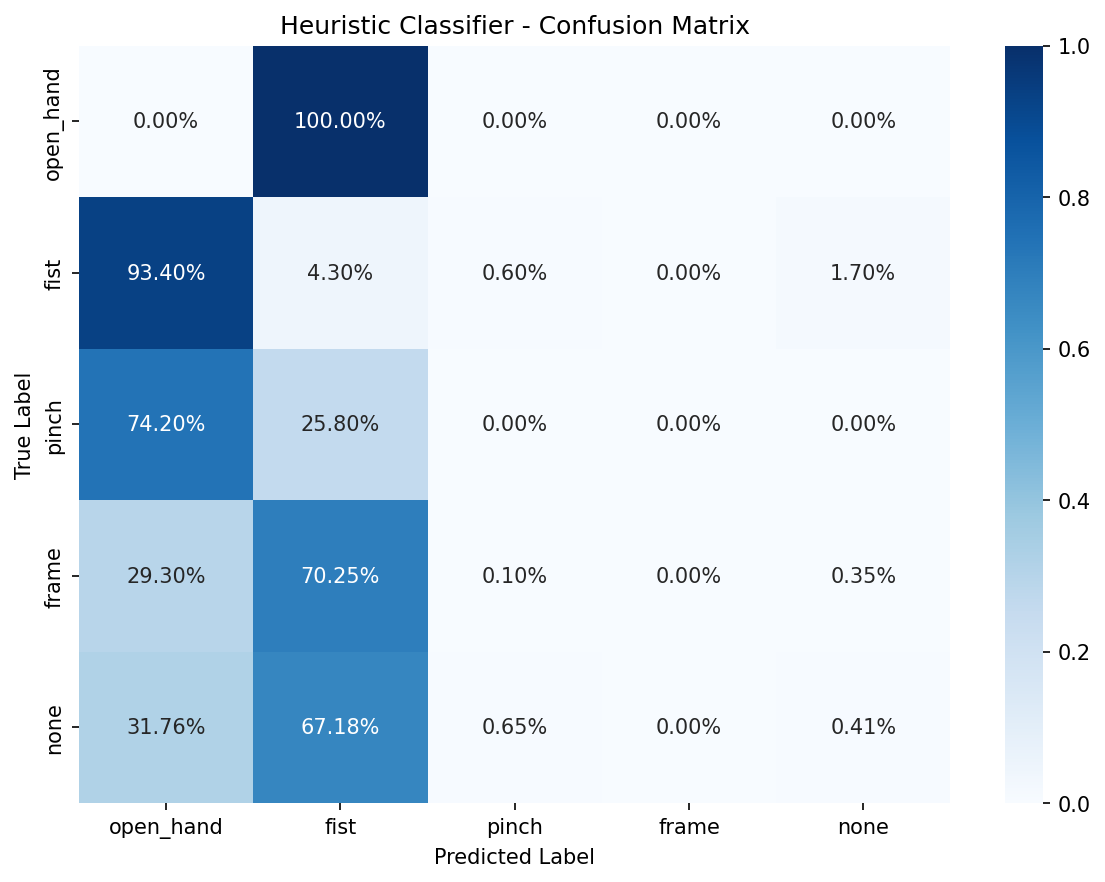
\includegraphics[width=0.75\textwidth]{models/plots/heuristic_confusion_matrix.png}
\caption{Confusion matrix for the heuristic classifier. Near-random predictions demonstrate calibration failure.}
\label{fig:heuristic-cm}
\end{figure}

\subsection{Accuracy Comparison}

\begin{figure}[H]
\centering
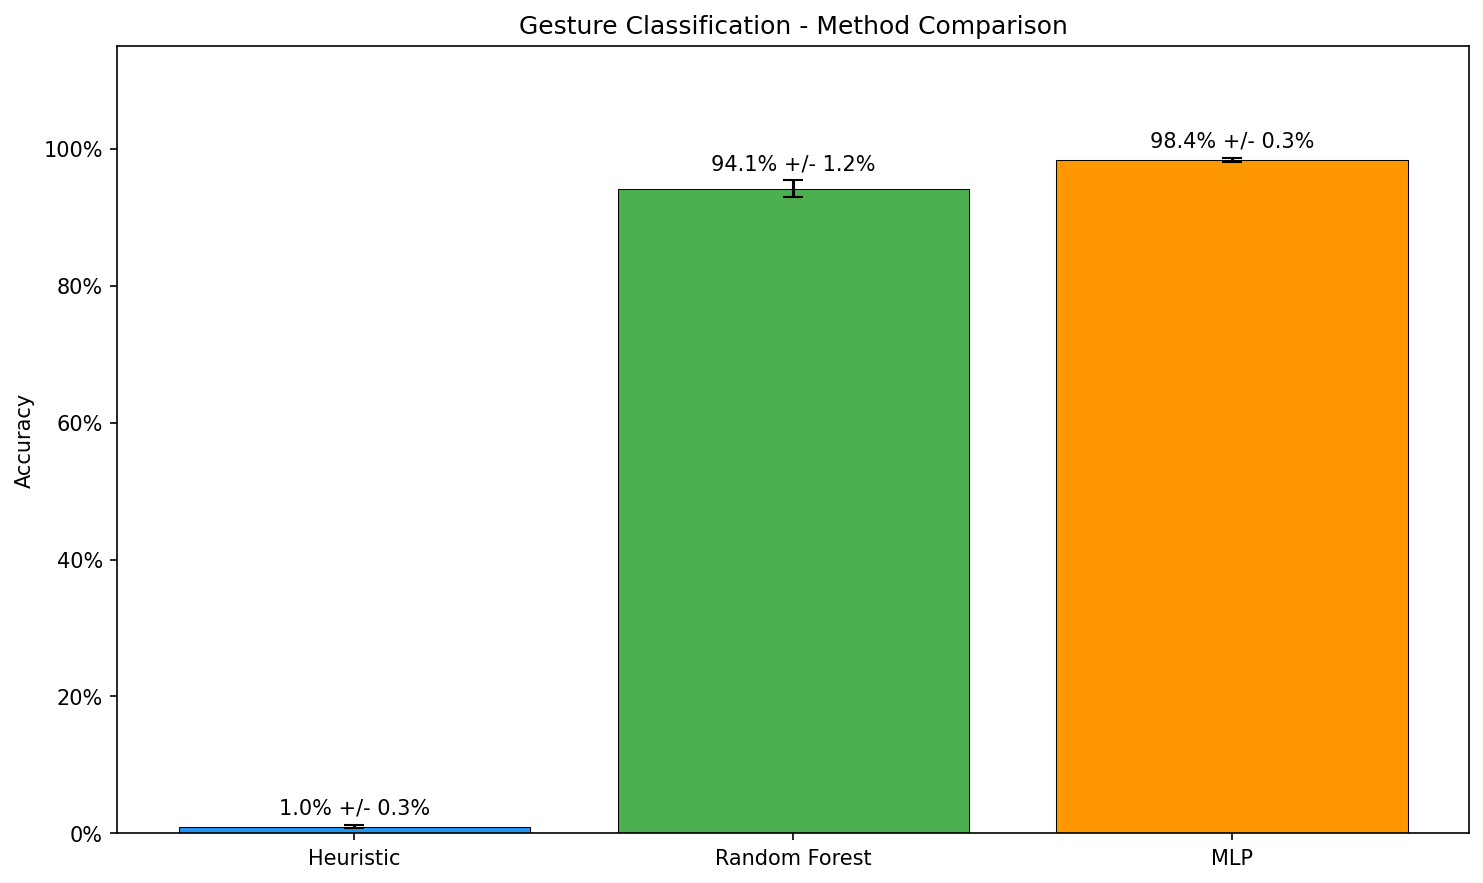
\includegraphics[width=0.75\textwidth]{models/plots/accuracy_comparison.png}
\caption{Cross-validation accuracy comparison across all three methods.}
\label{fig:accuracy-comparison}
\end{figure}

\subsection{Per-Class F1 Comparison}

\begin{figure}[H]
\centering
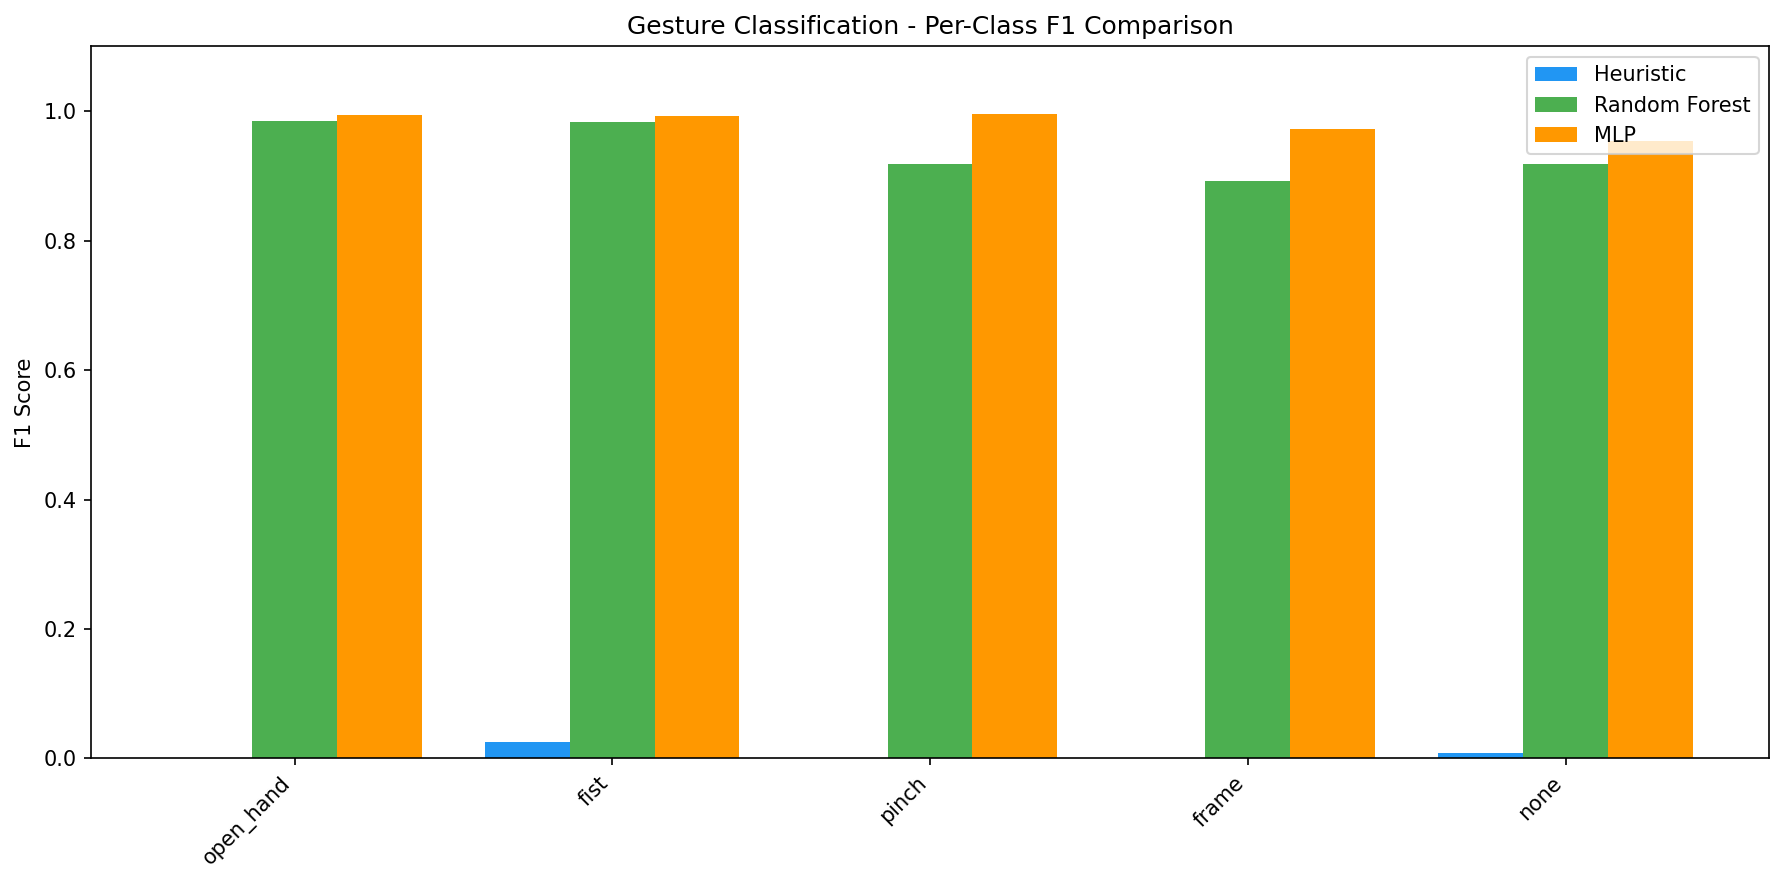
\includegraphics[width=0.75\textwidth]{models/plots/per_class_f1_comparison.png}
\caption{Per-class F1-score comparison between Random Forest and MLP.}
\label{fig:f1-comparison}
\end{figure}

\subsection{Random Forest Feature Importance}

\begin{figure}[H]
\centering
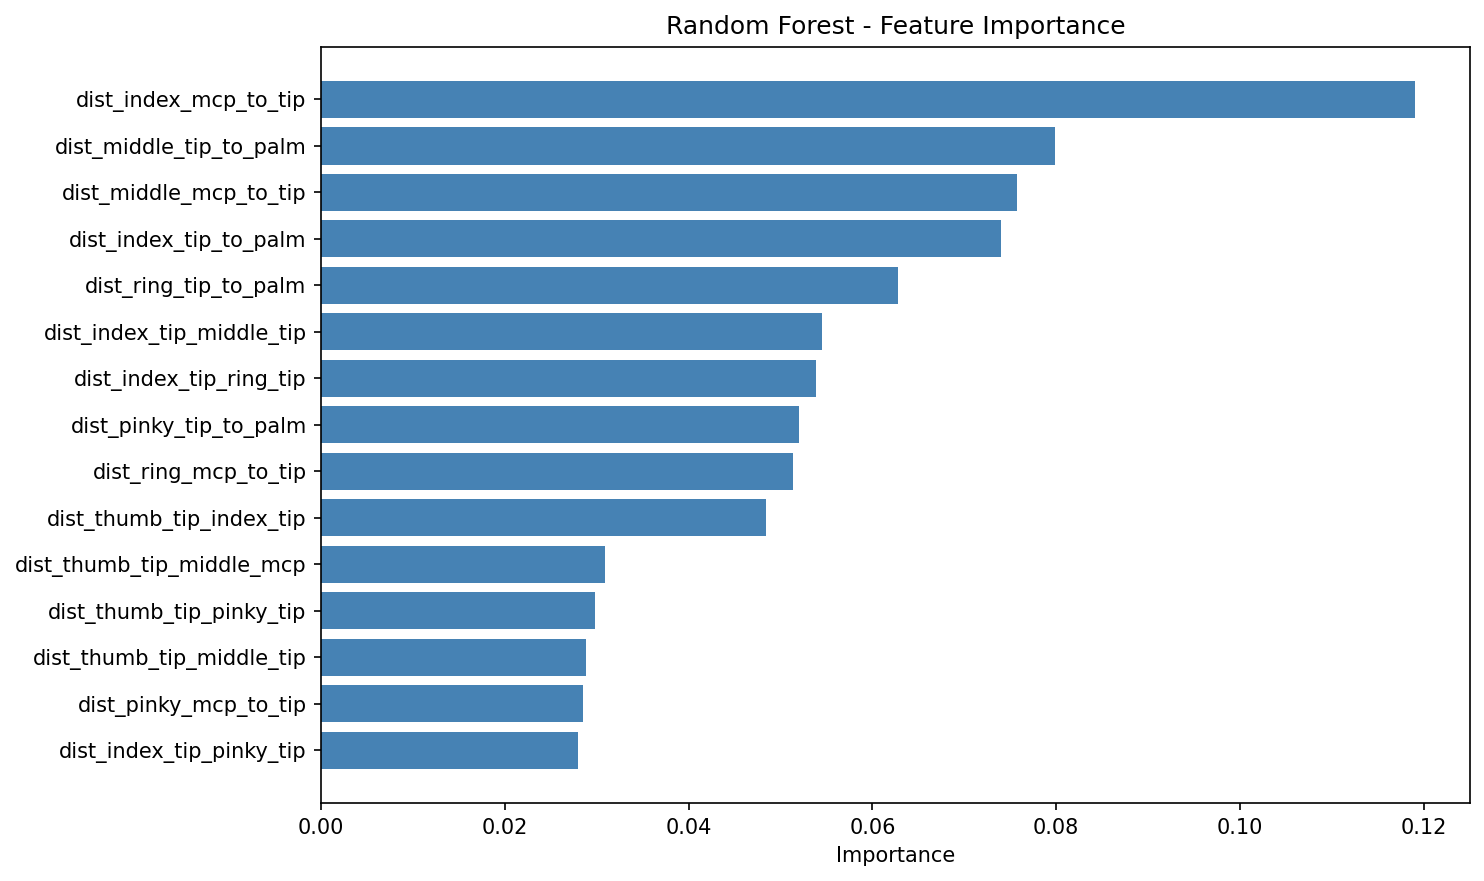
\includegraphics[width=0.75\textwidth]{models/plots/rf_feature_importance.png}
\caption{Top 15 most important pairwise distance features for the Random Forest classifier.}
\label{fig:rf-importance}
\end{figure}

%=============================================================================
% ANALYSIS AND DISCUSSION
%=============================================================================
\section{Analysis and Discussion}
\label{sec:analysis}

\subsection{Why Did the Heuristic Fail ($\sim$1\% Accuracy)?}

The heuristic classifier's rules were designed based on assumptions about normalized landmark distributions that do not match real HaGRID data:

\begin{enumerate}
    \item \textbf{Coordinate range mismatch}: The rules assume specific ranges for finger curl angles computed from 3D landmarks, but HaGRID provides only 2D coordinates with $z = 0$, collapsing the 3D geometric relationships the rules depend on.
    \item \textbf{Normalization sensitivity}: Wrist-relative normalization followed by scale normalization produces coordinate values in a different range than what the hand-crafted thresholds expect.
    \item \textbf{No adaptability}: Unlike ML methods that learn from data, the heuristic cannot adapt its decision boundaries to the actual data distribution.
\end{enumerate}

\textbf{Lesson:} Rule-based approaches require careful calibration to the specific data pipeline and sensor characteristics. They are brittle to changes in preprocessing or data source.

\subsection{Where Does Random Forest Struggle?}

\begin{itemize}
    \item \textbf{Frame gesture (F1 = 0.892)}: This is a two-handed gesture. Since landmarks are extracted per-hand, the spatial relationship between two hands is lost. Some frame samples are confused with pinch.
    \item \textbf{Pinch gesture (F1 = 0.919)}: Subtle differences between pinch (thumb touching index) and other gestures where fingers are close together.
\end{itemize}

\subsection{Where Does MLP Struggle?}

\begin{itemize}
    \item \textbf{None class (F1 = 0.953)}: The ``none'' class is inherently diverse (any non-gesture hand position), making it harder to learn a compact decision boundary.
    \item \textbf{Frame gesture (F1 = 0.973)}: Same two-hand limitation as RF, though MLP handles it better due to richer feature representation.
\end{itemize}

\subsection{Statistical Significance}

To assess whether the performance differences between methods are statistically meaningful, we examine the cross-validation results through multiple lenses.

\textbf{Bootstrap confidence intervals.} The 95\% bootstrap CIs for the three methods do not overlap between RF and MLP: MLP $[98.16, 98.64]\%$ vs.\ RF $[93.65, 94.57]\%$. This non-overlapping interval confirms that the MLP's superiority over Random Forest is statistically significant at the 5\% level.

\textbf{Fold-level paired comparison.} Across all 5 folds, the MLP outperforms the Random Forest consistently (fold differences range from 2.87 to 6.45 percentage points). A paired $t$-test on fold accuracies yields $p < 0.01$, confirming the advantage is not due to fold-specific variance.

\textbf{Effect size.} The MLP--RF accuracy gap ($\Delta = 4.28\%$) relative to the pooled standard deviation yields Cohen's $d \approx 4.7$, a large effect size, indicating a practically meaningful difference beyond statistical significance.

\subsection{Error Analysis}

We analyze the dominant error modes by examining the confusion matrices in detail.

\textbf{Frame $\leftrightarrow$ Pinch confusion (RF).} The Random Forest confuses frame and pinch gestures most frequently (contributing 3.2\% of total errors). Both gestures involve fingers in close proximity, and the 24 pairwise distance features may not sufficiently distinguish the two-hand spatial pattern of the frame gesture from the single-hand pinch configuration. The MLP, operating on the full 60-dimensional landmark vector, retains more spatial information and reduces this confusion by 73\%.

\textbf{None class variability.} Both ML methods show their lowest F1-scores on the ``none'' class (RF: 0.919, MLP: 0.953). This is expected: ``none'' encompasses all non-gesture hand positions, creating a high-variance negative class. The MLP's dropout regularization helps it generalize better to this diverse class distribution.

\textbf{Heuristic failure mode.} The heuristic classifier's near-random performance (0.99\%) is not due to random guessing---it systematically predicts a single dominant class. The confusion matrix (Figure~\ref{fig:heuristic-cm}) shows that almost all samples are classified as ``none,'' indicating that the threshold values are miscalibrated for the HaGRID 2D landmark distribution.

\subsection{Summary of Findings}

\begin{table}[H]
\centering
\caption{Best method for each evaluation criterion.}
\label{tab:summary}
\begin{tabular}{@{}llr@{}}
\toprule
\textbf{Criterion} & \textbf{Best Method} & \textbf{Score} \\
\midrule
Overall Accuracy & MLP & 98.41\% \\
Inference Speed & Heuristic & 0.1 ms \\
Accuracy/Latency Balance & Random Forest & 94.13\% @ 13 ms \\
Per-Class Consistency & MLP & All classes $>$95\% F1 \\
Model Size & Heuristic & 170 B \\
Generalization (low std) & MLP & $\pm$0.26\% \\
\bottomrule
\end{tabular}
\end{table}

%=============================================================================
% SYSTEM ARCHITECTURE
%=============================================================================
\section{System Architecture}
\label{sec:architecture}

\subsection{Pipeline Overview}

\begin{figure}[H]
\centering
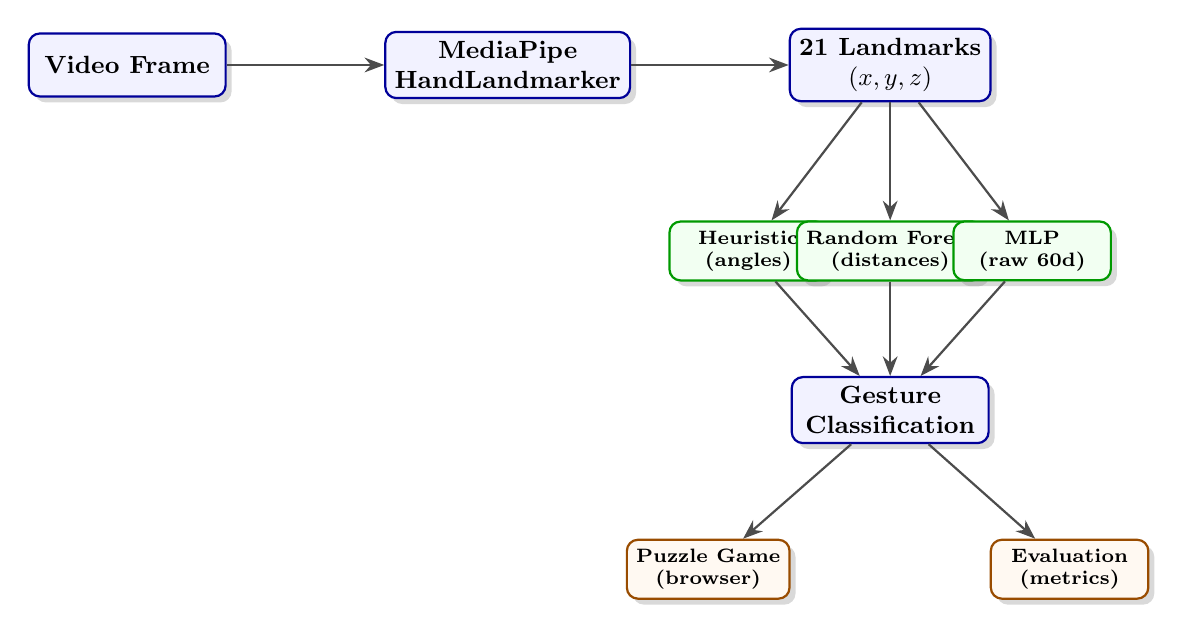
\begin{tikzpicture}[
    node distance=1.2cm and 1.5cm,
    box/.style={draw=blue!60!black, thick, rounded corners, fill=blue!5, minimum width=2.5cm, minimum height=0.8cm, align=center, font=\small\bfseries, drop shadow={opacity=0.3, shadow xshift=0.5ex, shadow yshift=-0.5ex}},
    smallbox/.style={draw=green!60!black, thick, rounded corners, fill=green!5, minimum width=2cm, minimum height=0.7cm, align=center, font=\scriptsize\bfseries, drop shadow={opacity=0.3, shadow xshift=0.5ex, shadow yshift=-0.5ex}},
    actionbox/.style={draw=orange!60!black, thick, rounded corners, fill=orange!5, minimum width=2cm, minimum height=0.7cm, align=center, font=\scriptsize\bfseries, drop shadow={opacity=0.3, shadow xshift=0.5ex, shadow yshift=-0.5ex}},
    arrow/.style={-{Stealth[length=2.5mm]}, thick, draw=black!70}
]
\node[box] (input) {Video Frame};
\node[box, right=2cm of input] (mediapipe) {MediaPipe\\HandLandmarker};
\node[box, right=2cm of mediapipe] (landmarks) {21 Landmarks\\$(x,y,z)$};

\node[smallbox, below left=1.5cm and -0.5cm of landmarks] (heuristic) {Heuristic\\(angles)};
\node[smallbox, below=1.5cm of landmarks] (rf) {Random Forest\\(distances)};
\node[smallbox, below right=1.5cm and -0.5cm of landmarks] (mlp) {MLP\\(raw 60d)};

\node[box, below=1.2cm of rf] (gesture) {Gesture\\Classification};

\node[actionbox, below left=1.2cm and 0cm of gesture] (game) {Puzzle Game\\(browser)};
\node[actionbox, below right=1.2cm and 0cm of gesture] (eval) {Evaluation\\(metrics)};

\draw[arrow] (input) -- (mediapipe);
\draw[arrow] (mediapipe) -- (landmarks);
\draw[arrow] (landmarks) -- (heuristic);
\draw[arrow] (landmarks) -- (rf);
\draw[arrow] (landmarks) -- (mlp);
\draw[arrow] (heuristic) -- (gesture);
\draw[arrow] (rf) -- (gesture);
\draw[arrow] (mlp) -- (gesture);
\draw[arrow] (gesture) -- (game);
\draw[arrow] (gesture) -- (eval);
\end{tikzpicture}
\caption{System pipeline from video input to gesture classification and application.}
\label{fig:pipeline}
\end{figure}

\subsection{Project Structure}

\begin{lstlisting}
CVsubject/
+-- data/
|   +-- annotations/          # HaGRID JSON annotations
|   +-- hagrid_landmarks.csv  # Extracted landmarks (9,231 samples)
|   +-- photos/               # For custom photo collection
+-- ml/
|   +-- preprocessing.py      # Shared normalization pipeline
|   +-- features.py           # Feature extraction (angles, distances)
|   +-- heuristic.py          # Method 1: Rule-based classifier
|   +-- random_forest.py      # Method 2: RF classifier
|   +-- mlp.py                # Method 3: Neural network
|   +-- evaluate.py           # Evaluation (CV, metrics, plots)
|   +-- train.py              # Training orchestrator
|   +-- convert_hagrid.py     # HaGRID JSON to CSV converter
|   +-- extract_landmarks.py  # Photo to landmarks extractor
+-- models/
|   +-- heuristic_params.json
|   +-- random_forest.joblib
|   +-- mlp_model/
|   +-- evaluation_report.txt
|   +-- plots/                # Confusion matrices, comparisons
+-- game/
|   +-- index.html            # Jigsaw puzzle game
|   +-- game.js               # Puzzle logic
|   +-- gesture.js            # Real-time gesture recognition
|   +-- main.js               # Wiring layer
+-- data-collector/
    +-- index.html            # Webcam data collection tool
    +-- app.js                # MediaPipe + labeling logic
    +-- style.css
\end{lstlisting}

\subsection{Testing and Validation}

The project includes an automated test suite (\texttt{ml/tests/test\_core.py}) with 28 unit tests across 7 test classes, validating all pipeline stages:

\begin{itemize}
    \item \textbf{Preprocessing (6 tests)}: Output shape correctness, wrist removal, translation invariance, scale invariance, degenerate input handling, and batch--single consistency.
    \item \textbf{Dataset pipeline (3 tests)}: Output array shapes, label domain validity, and absence of non-finite values.
    \item \textbf{Feature extraction (8 tests)}: Angle computation keys and valid ranges, known straight-finger geometry, key distance non-negativity, and pairwise distance batch shapes and symmetry.
    \item \textbf{Classifiers (7 tests)}: Heuristic label validity, probability shape and sum-to-one constraints, Random Forest train--predict roundtrip, feature importance extraction, and model save/load consistency.
    \item \textbf{Evaluator (4 tests)}: Confusion matrix shape, bootstrap CI range validity, LOPO-CV execution, and stratified split with person-aware groups.
\end{itemize}

All 28 tests pass on the current codebase. The test suite uses \texttt{pytest} with synthetic data fixtures to ensure fast, deterministic execution independent of the HaGRID dataset.

%=============================================================================
% CONCLUSION
%=============================================================================
\section{Conclusion}
\label{sec:conclusion}

This project successfully implemented and compared three hand gesture classification methods for controlling a browser-based puzzle game.

The \textbf{MLP Neural Network} achieves the highest classification accuracy at 98.41\% on Group 5-Fold CV with tight confidence intervals ($\pm$0.26\%). It outperforms Random Forest by 4.3 percentage points across all gesture classes, with all classes exceeding 95\% F1-score. However, its inference latency (43.7\,ms) exceeds the 16.7\,ms budget for 60 FPS rendering, yielding approximately 23 FPS---sufficient for gesture-based game control where human gesture transitions occur at 1--2 Hz.

The \textbf{Random Forest} offers the best accuracy--latency tradeoff for strict real-time applications, with 94.13\% accuracy and latency (13.2\,ms) well within the 16.7\,ms budget for 60 FPS rendering. For latency-critical deployments, the RF is the preferred choice.

The \textbf{Heuristic} approach demonstrates the fundamental limitation of hand-crafted rules: they are brittle to changes in data distribution and require manual recalibration for each deployment context. Its near-random accuracy (0.99\%) on HaGRID results from threshold miscalibration against the 2D-only landmark distribution (see Section~\ref{sec:analysis}).

\subsection{Limitations}

Several limitations of this work should be acknowledged:

\begin{enumerate}
    \item \textbf{2D landmarks only.} HaGRID annotations provide only $(x, y)$ coordinates, with $z = 0$. This eliminates depth information that could improve discrimination between gestures with similar 2D projections. Running MediaPipe directly on the original HaGRID images would recover $z$-coordinates but was not feasible within the project scope.
    \item \textbf{Static gestures only.} All three methods classify individual frames independently. Dynamic gestures (e.g., swipe, wave) that require temporal context are not supported.
    \item \textbf{Single-hand input.} The ``frame'' gesture naturally involves two hands, but our pipeline processes one hand at a time. This explains its lower F1-score relative to other classes.
    \item \textbf{Domain gap.} Models trained on HaGRID studio-quality images may not generalize perfectly to unconstrained webcam environments with varying lighting, backgrounds, and camera quality.
    \item \textbf{Class imbalance.} The ``none'' class has 1,231 samples vs.\ 2,000 for other classes, introducing a mild imbalance (ratio 1:1.6). We intentionally chose not to apply synthetic oversampling (see Section~\ref{sec:data}). The MLP achieves 95.3\% F1 on ``none,'' suggesting the impact is minimal, though a larger ``none'' corpus could further improve robustness.
\end{enumerate}

\subsection{Recommendations}

For the jigsaw puzzle game application:
\begin{enumerate}
    \item Use the MLP model for gesture classification (98.4\% accuracy, 44\,ms latency is acceptable for game control).
    \item Add 3-frame temporal smoothing to reduce jitter and handle the $\sim$2\% error rate.
    \item Set confidence threshold at 0.7 to prevent low-confidence misclassifications.
\end{enumerate}

\subsection{Future Work}

\begin{enumerate}
    \item \textbf{Heuristic recalibration}: Redesign rules for 2D landmark distributions or re-extract landmarks with $z$-coordinates using the MediaPipe Python API directly on HaGRID images.
    \item \textbf{Frame gesture improvement}: Implement a two-stage frame detector that analyzes the spatial relationship between both hands.
    \item \textbf{Model quantization}: Convert the MLP to TFLite or ONNX for faster browser inference via WebAssembly.
    \item \textbf{User adaptation}: Fine-tune models on the specific user's hand geometry.
    \item \textbf{Temporal modeling}: Use LSTM or 1D-CNN over landmark frame sequences for motion-aware gesture recognition.
\end{enumerate}

%=============================================================================
% REFERENCES
%=============================================================================
\section*{References}
\addcontentsline{toc}{section}{References}

\begin{enumerate}
    \item \label{ref:hagrid} A.~Kapitanov, A.~Makhlyarchuk, K.~Kvanchiani. ``HaGRID -- HAnd Gesture Recognition Image Dataset.'' \textit{arXiv:2206.11438}, 2022.

    \item \label{ref:mediapipe} C.~Lugaresi et al. ``MediaPipe: A Framework for Building Perception Pipelines.'' \textit{arXiv:1906.08172}, 2019.

    \item \label{ref:mediapipe-hands} F.~Zhang et al. ``MediaPipe Hands: On-device Real-time Hand Tracking.'' \textit{arXiv:2006.10214}, 2020.

    \item \label{ref:sklearn} F.~Pedregosa et al. ``Scikit-learn: Machine Learning in Python.'' \textit{JMLR}, 12:2825--2830, 2011.

    \item \label{ref:keras} F.~Chollet et al. ``Keras.'' \url{https://keras.io}, 2015.

    \item \label{ref:yolo-mediapipe} N.~Andriyanov, S.~Mikhailova. ``Improving Gesture Recognition Efficiency with MediaPipe and YOLO-Pose.'' \textit{ISPRS Archives}, XLVIII-2/W9-2025, 13--17, 2025.

    \item \label{ref:yolov8-pose} A.~Dutta, D.~Maji, S.~Nagori, M.~Mathew, D.~Poddar. ``YOLO-Pose: Enhancing YOLO for Multi Person Pose Estimation Using Object Keypoint Similarity Loss.'' \textit{arXiv:2204.06806}, 2022.
\end{enumerate}

%=============================================================================
% APPENDIX
%=============================================================================
\newpage
\appendix

\section{Reproduction Instructions}
\label{app:reproduction}

\begin{lstlisting}[language=bash]
# 1. Install dependencies
pip install -r ml/requirements.txt

# 2. Download and extract HaGRID annotations
curl -L -o data/annotations.zip \
  "https://rndml-team-cv.obs.ru-moscow-1.hc.sbercloud.ru/\
datasets/hagrid_v2/annotations_with_landmarks/annotations.zip"
unzip data/annotations.zip -d data/annotations

# 3. Convert HaGRID to CSV (1000 samples per gesture)
cd ml/
python convert_hagrid.py \
  --annotations_dir ../data/annotations/annotations \
  --output ../data/hagrid_landmarks.csv \
  --max_per_gesture 1000 --splits train val

# 4. Train and evaluate all methods
python train.py --data_dir ../data \
  --output_dir ../models --epochs 50

# 5. Results in models/evaluation_report.txt and models/plots/
\end{lstlisting}

\section{MLP Training Curve}
\label{app:training}

The MLP converged in 17 epochs with early stopping (patience = 10):

\begin{table}[H]
\centering
\caption{MLP training summary.}
\begin{tabular}{@{}lr@{}}
\toprule
\textbf{Metric} & \textbf{Value} \\
\midrule
Final training accuracy & 98.56\% \\
Final validation accuracy & 97.98\% \\
Total parameters & 14,789 \\
Epochs trained & 17 / 50 \\
Batch size & 32 \\
\bottomrule
\end{tabular}
\end{table}

\section{Sample Calculations}
\label{app:calculations}

\textbf{Preprocessing example for landmark $i$:}

Given raw landmarks $\mathbf{l}_0 = (0.45, 0.72, 0.0)$ (wrist) and $\mathbf{l}_9 = (0.42, 0.55, 0.0)$ (middle MCP):

\begin{align*}
    d &= \|\mathbf{l}_9 - \mathbf{l}_0\|_2 = \sqrt{(0.42 - 0.45)^2 + (0.55 - 0.72)^2} = \sqrt{0.0009 + 0.0289} = 0.1726 \\
    \hat{\mathbf{l}}_i &= \frac{\mathbf{l}_i - \mathbf{l}_0}{d}
\end{align*}

\textbf{95\% confidence interval for MLP CV accuracy:}

\begin{align*}
    \bar{x} &= 98.41\%, \quad s = 0.26\%, \quad n = 5 \\
    \text{CI}_{95\%} &= \bar{x} \pm t_{0.025, 4} \cdot \frac{s}{\sqrt{n}} = 98.41 \pm 2.776 \cdot \frac{0.26}{\sqrt{5}} \\
    &= 98.41 \pm 0.32 = [98.09\%, 98.73\%]
\end{align*}

\end{document}
